\documentclass{article}

\usepackage{graphicx}

\title{Effect Network - Decentralised network for Artificial Intelligence \\ \vspace{16pt} \large \textbf{DRAFT}}
\date{\today}
\author{Jesse Eisses, Laurens Verspeek \\
  \small \texttt{\{jeisses, lverspeek\}@itsavirus.com}}

\begin{document}

\maketitle

\begin{abstract}

\end{abstract}

\section{Introduction}
In the past half-decade there has been a rapid growth in the number of
practical Artificial Intelligence applications around us. Smart
services, like self-driving cars, face and voice recognition in mobile
phones and image translation are getting a central place in everyday
life. This rise can be explained by the recent advances in machine
learning research in combination with the large adoption from the
industry. While the academic achievements are available to the public,
most applied AI algorithms are developed and run at large corporations
behind closed doors. Three major reasons that make the development
inaccessible for individuals are given below:

\begin{description}
\item[Data processing] A common property of intelligent applications
  is that they perform tasks that traditionally require human
  feedback. Such tasks involve processing unstructured data and
  finding a pattern that can be used to provide useful output. These
  applications are trained on large datasets with annotations. Obtaining
  an annotated dataset is non-trivial and requires a lot of time and
  money.
  
  \emph{Effect} introduces a micro-tasking platform that connects a 
  large task-force of workers to any entity that requires human feedback 
  on some form of data of any size. This is explained in Section \ref{sec:phase1}.
  
\item[Diverging tasks] An obstacle when developing a complex
  algorithm is the need to interact with parts of the world outside
  the current domain. For example: a self-driving car learning to steer 
  will also need to identify road signs around the world. This
  situation can best be treated as a knowledge system where the
  classification of the sign is done by an external application. This
  quickly increases the amount of work needed.
  
  The \emph{Effect Network} is an exchange with a rich ontology of 
  specialist AI applications. Individual applications can find each 
  other to buy or sell information, as specified in section x.
  
\item[Computational cost] Developing and training a large AI is a
  computational intensive task, and requires a technical
  infrastructure capable of processing terabytes of data, doing
  batched processing on multiple GPUs and coordinating the results. 
  
  \emph{Effect} proposes a system to train and run intelligent 
  algorithms in a distributed fashion in section x.
\end{description}

To make the development of AI applications more accessible, and to
stimulate their growth and freedom, we propose a private,
decentralized ecosystem called the \emph{Effect Network}. The network
is designed to provide a fully decentralized alternative to the
markets shown in table~\ref{tab:service_compare}. The decentralization
is achieved by running on a blockchain that supports Turning-complete
smart contracts.\\


\begin{table}
  \centering
  \begin{tabular}[h]{l|l|l}
    \textbf{Market} & \textbf{Suppliers} & \textbf{Market Cap.} \\ \hline
    Micro tasking & Amazone Mechanical Turk, Fiverr, \dots & \dots \\ 
    AI as a service & Watson, Amazon Rekognition, \dots & \dots \\
    Computational platform & Google Cloud ML, Amazone AI, \dots & \dots 
  \end{tabular}
  \caption{Overview of markets (WIP)}\label{tab:service_compare}
\end{table}

The \emph{Effect Network}, like other decentralized applications,
directly connects supply and demand without the need for an
intermediary party. Competitive prices \dots\\

The \emph{Effect Network} will significantly improve the global Artificial Intelligence market:
\begin{itemize}
    \item \textbf{Accessibility.} By directly linking supply and demand through our micro-tasking platform (see Section \ref{sec:phase1}) the \emph{Effect Network} will make training AI algorithms easier, faster and cheaper. This will enable people who don't have access to a large dataset or a big network to train their AI algorithm.
    \item \textbf{Accuracy.} The \emph{Effect Network} is an exchange with a rich ontology of specialist AI applications. Individual applications can find each 
  other to buy or sell information, as specified in Section \ref{sec:phase2}. Through this exchange users can use data sets with significantly higher complexities to train their AI algorithms.
    \item \textbf{Performance.} People can directly buy existing datasets on the \emph{Effect Exchange} (Section \ref{sec:phase2}) or quickly create their own dataset by creating micro-task on the \emph{Effect Mechanical Turk} platform (Section \ref{sec:phase1}). By enabling people to retrieve accurate datasets quickly, they can immediately use these datasets to train AI Algorithms.
    \item \textbf{Interoperability.} By putting the AI algorithms on the blockchain and creating a standard to which these AI algorithms have to comply to, we can truly decentralize AI and achieve interoperability between individual AIs. The combination of multiple AI algorithms will result in powerful capabilities and emergent intelligence that no single AI algorithm can achieve on his own. 
\end{itemize}

\section{Decentralized Mechanical Turk}
\label{sec:phase1}
The \emph{Effect Mechanical Turk} platform is a decentralized, peer to
peer marketplace for work that requires human intelligence.  It
provides similar features as centralized services like Amazon
Mechanical Turk\footnote{}, Fiverr\footnote{}, Crowdsource\footnote{}
and Guru.com\footnote{}. It is a crowd sourcing technology that
enables requesters to submit tasks that can be completed by human
agents in exchange for compensation. Users can work on tasks from
requesters at any time, anywhere and from any device. The task are
called Human Intelligence Tasks or HIT’s for short. The providers of
the HIT’s are called \emph{requesters}. When a user completes a task,
they are paid with with a network token called AIX.

\subsection{Tasks}
In essence a task involves providing feedback on a (multi-)media
asset. A task has the following properties:

\begin{table}[h]
  \centering
  \begin{tabular}[h]{r|l}
    Dataset & URL \\
    Description & description of the task \\ 
    Contract ID & smart contract that will handle task \\
    Blueprint & data for the contract \\ 
    Required \emph{honor} & require trusted users \\
    Reward & rewarded AIX upon completion \\
    Num. ratings & number of ratings per user \\
    Rating timeout & timeout on performing a rating \\ 
    Expiration  & block ID after which task expires \\
    Sequence id & for sequencing examples (optional)\\
    Data credentials & to unlock private datasets \\
  \end{tabular}
  \caption{Properties of a task}
  \label{tab:task}
\end{table}

A task refers to a dataset that can contain any amount of media
assets. The contract ID of the task will validate the format of the
data. Extracting and presenting examples form the dataset is done by
the user interface.

The structure and required feedback for a task are defined by the
contract ID and the blueprint.

\subsection{Media}
Media assets are often large and of varying form. A blockchain is not
a suitable database for storing this kind of information. Other
decentralized storage options, like BitTorrent\footnote{} and
IPFS\footnote{}, are specialized in these types of assets. For this
reason the network will use such a hash-based distributed file
storage, where each media asset can be revered to by a single hash.

Note that the feedback on a \emph{task} can also involve storing media
assets, for example during image segmentation. In this case the
ratings asset will be stored on the distributed storage, and a hash
and checksum of the rating are stored on the blockchain.

Requesters will also be able to supply datasets through traditional
channels, like Amazone S3, Google Cloud Storage and FTP.

\subsection{Privacy}
The blockchain is decentralized and open by nature. There are several
measures that must be taken to make sure the Effect network can be
used for vulnerable information. The network can provide privacy for
the following cases:

\begin{description}
\item[Datasets] Requesters can provide their dataset in encrypted
  form. Only selected users will be able to decrypt or access the
  data. This is determined by network smart contracts using Public Key
  Encryption, where selected users can decrypt the dataset
  credentials.
\item[User ratings] Tasks can be made anonymous, so that feedback can
  not be traced back to a specific user.
\end{description}

Tasks that involve privacy features will be more computational
expensive, thus will also have a higher network fee.

\section{Decentralized AI Services}
\label{sec:phase2}
- exchange with a rich ontology of specialist AI applications. Individual applications can find each other to buy or sell information\dots -

\section{Decentralized AI Algorithms}
\label{sec:phase3}
- Put AI algorithms on the blockchain. The algorithms can interact with each other\dots -

\section{Community}
The described network can be deployed and used as a decentralized
application as-is. However, in order for the network to grow and be
sustainable, we believe there has to be a form of governance. Parties
should have incentive to use the AIX token for the purpose AI
tasks. Investors looking for quick monetary gain should be discouraged
and pump-and-dump schemes should be avoided, in order for the network
to grow and slowly take market value from the existing centralized
services.

\begin{figure}[htb]
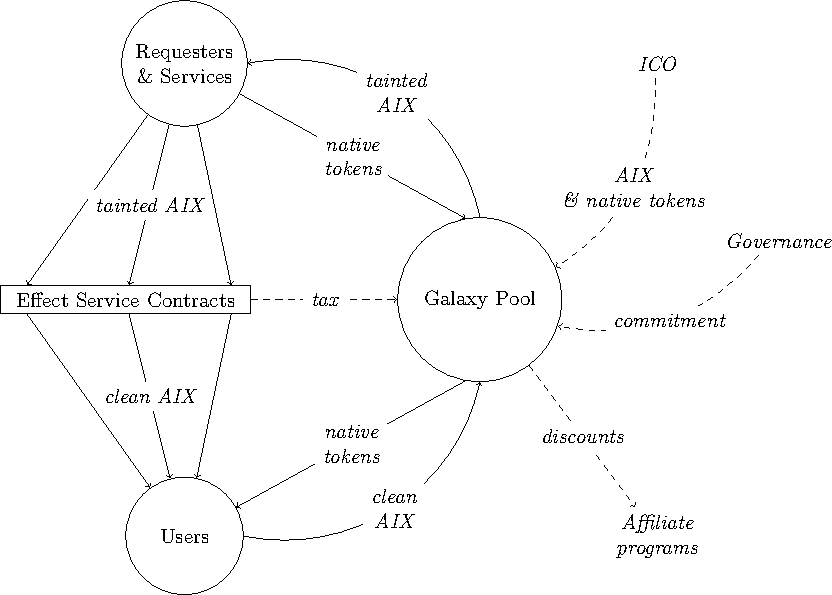
\includegraphics[width=\textwidth]{pictures/galaxy.pdf}
\caption{Diagram of the relation between the different Effect
  Community elements.}
\end{figure}

\subsection{AIX and the Galaxy Pool}
It is important to maintain liquidity in AIX, especially during the
early days when there is no listing on exchanges. Ideally the
following rules should always hold at all times:

\begin{enumerate}
\item Workers are able to sell their AIX rewards for native tokens
\item Requesters and network users are able to buy AIX
\end{enumerate}

For a new token on the market this kind of liquidity can be hard to
achieve and can be hurt by speculative trading.

The Effect Network will maintain a central pool of tokens to provide
liquidity, encourage adoption and stabilize network fees. This
reservoir is called the Galaxy Pool and consists of a mix of AIX and
native tokens. Several rules will drive the Galaxy Pool towards an
equilibrium. These rules can be later be refined by means of
governance as is discussed in section~\ref{sec:governance}.

The Galaxy Pool ensures stable exchange rates for users of the
platform at all times. The pool is not suitable for day traders, as
only \emph{tainted} coins can be bought.

\subsection{Honor Tokens and Fraud}
\label{sec:fraud}
The honor token is a token that can not be traded

\subsection{Proof of Commitment and Governance}
\label{sec:governance}

\section{Examples}

\section{Note on Ethics}

\end{document}